\documentclass[a4paper]{jpconf}
\usepackage{graphicx}
\usepackage{comment}
\usepackage{cite}
\usepackage{gensymb}


\begin{document}


\title{Validation of an Actuator Line Model Coupled to a Dynamic Stall Model for
Pitching Motions Characteristic to Vertical Axis Turbines}


\author{Victor Mendoza$^{1}$, Peter Bachant$^{2}$, Martin Wosnik$^{2}$ and Anders Goude$^{1}$ }
\address{$^{1}$ Department of Engineering Sciences, Division of Electricity, Uppsala University, \\Uppsala 751 21, Sweden}
\address{$^{2}$ Center for Ocean Renewable Energy, University of New Hampshire, 24 Colovos Rd.,\\ Durham, NH 03824, USA}
\ead{victor.mendoza@angstrom.uu.se}


\begin{abstract}

    Vertical axis turbines (VATs) can be used to extract renewable energy from
    wind or water flows. A simpler design, low cost of maintenance, and the
    ability to accept flow from all directions perpendiculat to the rotor axis
    are some of the most important advantages over conventional horizontal axis
    turbines (HATs). However, VATs encounter complex and unsteady fluid
    dynamics, which present significant modeling challenges. One of the most
    relevant phenomena is dynamic stall, which is caused by the unsteady
    variation of angle of attack throughout the blade rotation, and is the focus
    of the present study. Dynamic stall is usually used as a passive control for
    VAT operating conditions, hence the importance of predicting its effects. In
    this study, \textbf{a coupled model is implemented with the open-source CFD
    toolbox OpenFOAM for solving the Navier--Stokes equations, where an actuator
    line model and dynamic stall model are used compute the blade loading and
    body force.} Force coefficients obtained from the model are validated with
    experimental data of pithing airfoil in similar operating conditions as
    H-rotor type. Numerical results show reasonable agreement with experimental
    data for pitching motion.

\end{abstract}


\section{Introduction}

Operating conditions of VAWTs are characterized as complex unsteady flows which
give a considerable challenge, both to describe using measurements and to
represent through simulation tools\cite{huyer1996unsteady}. Moreover, VAWT
blades are inherently exposed to cyclic variation in the angle of attack, which
gives cyclic blade forces and can give material fatigue damage. Accurate
modeling of the varying forces is therefore very important for the design of the
VAWT.

The amplitude of the angle of attack oscillation in a fixed pitch VAWT is increasing
with decreased tip speed
ration (TSR), and at low TSR (common during stall regulation), the blades will
experience dynamic stall, where the force coefficients for the blade not only
depend on the angle of attack, but also on the rate of change of the angle of
attack. The aim of this study is to investigate the performance of a
Leishman-Beddoes type dynamic stall model when implemented within an actuator
line model, for pitching motion typical to a VAWT.


\section{Methodology}

For solving the governing equations of the phenomena involved, a coupled model have
been implemented: the actuator line model is used to calculate the flow
velocities and thereby the angle of attack. The dynamic stall model is used to
calculate blade force coefficients, which the actuator line model needs for the
velocity field calculations.

In this work, it was chosen to validate the model
against wind tunnel data for a pitching blade. This will put the focus on the
force modeling part in the simulation model.

\textbf{Actuator Line Model:} is a three-dimensional and unsteady aerodynamic
model developed by S{\o}rensen and Shen\cite{sorensen1999computation}, used to
study the flow around wind turbines. It is a combination of a solver of
Navier-Stokes equations with a so-called actuator line technique, in which
blades of the turbine are represented by a radial distribution of body forces
along lines. These forces are determined using a dynamic stall model commonly
based on empirical data. This work uses the library turbinesFoam developed by
Bachant\cite{bachant2015simulating}.

\textbf{Dynamic Stall Modeling:} is represented by the Leishman-Beddoes
model\cite{leishman1986generalised} with the modifications of Sheng et
al\cite{sheng2008modified} and Dyachuk\cite{dyachuk}.
It is capable to calculate the unsteady lift,
pitching moment and drag, giving a physical description of the aerodynamics. It
have been validated with experimental data in\cite{leishman1989semi}.
The model is separated into three subsystems: an attached flow model for unsteady linear
airloads, a separated flow model for non-linear airloads and a dynamic stall
model for the airloads induced by the leading edge vortex.

A NACA0021 airfoil was tested at the Reynolds number of 1.000.000 (which is a
reasonable value for operating VAWT) during pithing motion similar to the motion
of the VAWT blade. Different pitching amplitudes were investigated. In a VAWT with
fixed blades, the angle of attack is in function of the TSR of the turbine. A
periodic function is used to represent the variations of the angles of attack
which a VAWT blade experiences analog to the pitching motion,
\begin{eqnarray}
    \alpha = \arctan \left( \frac{\sin \theta}{\lambda + \cos \theta} \right),
\end{eqnarray}
where $\theta$ is the azimuthal blade angle and $ \lambda $ represents the TSR,
\begin{eqnarray}
    \lambda =  \frac{\Omega R}{V}.
\end{eqnarray}
The pitching blade experiments were carried out at Glasgow
University\cite{angell1988collected}.\\

\begin{figure}[h]
\begin{minipage}{18pc}
%\includegraphics[width=18pc]{Fig1.png}
\resizebox{\columnwidth}{!}{% GNUPLOT: LaTeX picture with Postscript
\begingroup
  \makeatletter
  \providecommand\color[2][]{%
    \GenericError{(gnuplot) \space\space\space\@spaces}{%
      Package color not loaded in conjunction with
      terminal option `colourtext'%
    }{See the gnuplot documentation for explanation.%
    }{Either use 'blacktext' in gnuplot or load the package
      color.sty in LaTeX.}%
    \renewcommand\color[2][]{}%
  }%
  \providecommand\includegraphics[2][]{%
    \GenericError{(gnuplot) \space\space\space\@spaces}{%
      Package graphicx or graphics not loaded%
    }{See the gnuplot documentation for explanation.%
    }{The gnuplot epslatex terminal needs graphicx.sty or graphics.sty.}%
    \renewcommand\includegraphics[2][]{}%
  }%
  \providecommand\rotatebox[2]{#2}%
  \@ifundefined{ifGPcolor}{%
    \newif\ifGPcolor
    \GPcolorfalse
  }{}%
  \@ifundefined{ifGPblacktext}{%
    \newif\ifGPblacktext
    \GPblacktexttrue
  }{}%
  % define a \g@addto@macro without @ in the name:
  \let\gplgaddtomacro\g@addto@macro
  % define empty templates for all commands taking text:
  \gdef\gplbacktext{}%
  \gdef\gplfronttext{}%
  \makeatother
  \ifGPblacktext
    % no textcolor at all
    \def\colorrgb#1{}%
    \def\colorgray#1{}%
  \else
    % gray or color?
    \ifGPcolor
      \def\colorrgb#1{\color[rgb]{#1}}%
      \def\colorgray#1{\color[gray]{#1}}%
      \expandafter\def\csname LTw\endcsname{\color{white}}%
      \expandafter\def\csname LTb\endcsname{\color{black}}%
      \expandafter\def\csname LTa\endcsname{\color{black}}%
      \expandafter\def\csname LT0\endcsname{\color[rgb]{1,0,0}}%
      \expandafter\def\csname LT1\endcsname{\color[rgb]{0,1,0}}%
      \expandafter\def\csname LT2\endcsname{\color[rgb]{0,0,1}}%
      \expandafter\def\csname LT3\endcsname{\color[rgb]{1,0,1}}%
      \expandafter\def\csname LT4\endcsname{\color[rgb]{0,1,1}}%
      \expandafter\def\csname LT5\endcsname{\color[rgb]{1,1,0}}%
      \expandafter\def\csname LT6\endcsname{\color[rgb]{0,0,0}}%
      \expandafter\def\csname LT7\endcsname{\color[rgb]{1,0.3,0}}%
      \expandafter\def\csname LT8\endcsname{\color[rgb]{0.5,0.5,0.5}}%
    \else
      % gray
      \def\colorrgb#1{\color{black}}%
      \def\colorgray#1{\color[gray]{#1}}%
      \expandafter\def\csname LTw\endcsname{\color{white}}%
      \expandafter\def\csname LTb\endcsname{\color{black}}%
      \expandafter\def\csname LTa\endcsname{\color{black}}%
      \expandafter\def\csname LT0\endcsname{\color{black}}%
      \expandafter\def\csname LT1\endcsname{\color{black}}%
      \expandafter\def\csname LT2\endcsname{\color{black}}%
      \expandafter\def\csname LT3\endcsname{\color{black}}%
      \expandafter\def\csname LT4\endcsname{\color{black}}%
      \expandafter\def\csname LT5\endcsname{\color{black}}%
      \expandafter\def\csname LT6\endcsname{\color{black}}%
      \expandafter\def\csname LT7\endcsname{\color{black}}%
      \expandafter\def\csname LT8\endcsname{\color{black}}%
    \fi
  \fi
  \setlength{\unitlength}{0.0500bp}%
  \begin{picture}(7200.00,5040.00)%
    \gplgaddtomacro\gplbacktext{%
      \csname LTb\endcsname%
      \put(946,704){\makebox(0,0)[r]{\strut{}-1.5}}%
      \csname LTb\endcsname%
      \put(946,1383){\makebox(0,0)[r]{\strut{}-1}}%
      \csname LTb\endcsname%
      \put(946,2061){\makebox(0,0)[r]{\strut{}-0.5}}%
      \csname LTb\endcsname%
      \put(946,2740){\makebox(0,0)[r]{\strut{} 0}}%
      \csname LTb\endcsname%
      \put(946,3418){\makebox(0,0)[r]{\strut{} 0.5}}%
      \csname LTb\endcsname%
      \put(946,4097){\makebox(0,0)[r]{\strut{} 1}}%
      \csname LTb\endcsname%
      \put(946,4775){\makebox(0,0)[r]{\strut{} 1.5}}%
      \csname LTb\endcsname%
      \put(1078,484){\makebox(0,0){\strut{}-20}}%
      \csname LTb\endcsname%
      \put(1794,484){\makebox(0,0){\strut{}-15}}%
      \csname LTb\endcsname%
      \put(2509,484){\makebox(0,0){\strut{}-10}}%
      \csname LTb\endcsname%
      \put(3225,484){\makebox(0,0){\strut{}-5}}%
      \csname LTb\endcsname%
      \put(3941,484){\makebox(0,0){\strut{} 0}}%
      \csname LTb\endcsname%
      \put(4656,484){\makebox(0,0){\strut{} 5}}%
      \csname LTb\endcsname%
      \put(5372,484){\makebox(0,0){\strut{} 10}}%
      \csname LTb\endcsname%
      \put(6087,484){\makebox(0,0){\strut{} 15}}%
      \csname LTb\endcsname%
      \put(6803,484){\makebox(0,0){\strut{} 20}}%
      \put(176,2739){\rotatebox{-270}{\makebox(0,0){\strut{}$C_N$}}}%
      \put(3940,154){\makebox(0,0){\strut{}Angle of attack {$\alpha$} [$\degree$]}}%
    }%
    \gplgaddtomacro\gplfronttext{%
      \csname LTb\endcsname%
      \put(4437,4602){\makebox(0,0)[r]{\strut{}$C_N$ simulated}}%
      \csname LTb\endcsname%
      \put(4437,4382){\makebox(0,0)[r]{\strut{}$C_N$ experiments}}%
    }%
    \gplbacktext
    \put(0,0){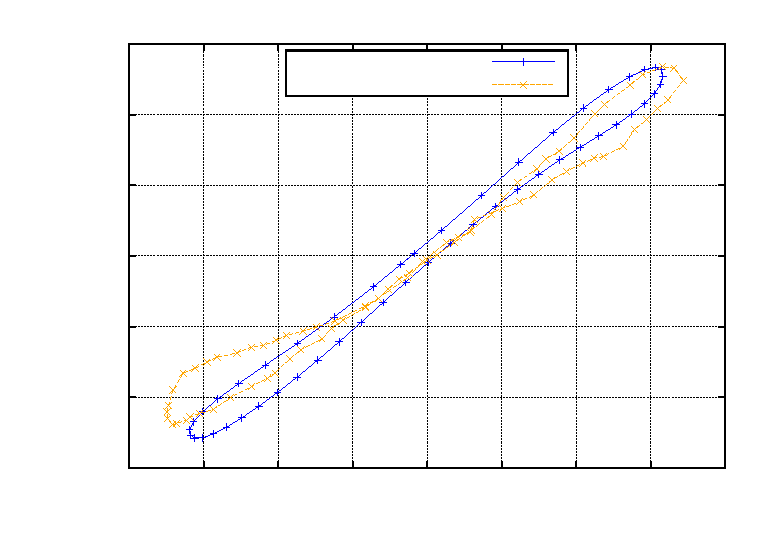
\includegraphics{CN1}}%
    \gplfronttext
  \end{picture}%
\endgroup
}
\end{minipage}\hspace{2pc}%
\begin{minipage}{18pc}
%\includegraphics[width=18pc]{Fig2.png}
\resizebox{\columnwidth}{!}{% GNUPLOT: LaTeX picture with Postscript
\begingroup
  \makeatletter
  \providecommand\color[2][]{%
    \GenericError{(gnuplot) \space\space\space\@spaces}{%
      Package color not loaded in conjunction with
      terminal option `colourtext'%
    }{See the gnuplot documentation for explanation.%
    }{Either use 'blacktext' in gnuplot or load the package
      color.sty in LaTeX.}%
    \renewcommand\color[2][]{}%
  }%
  \providecommand\includegraphics[2][]{%
    \GenericError{(gnuplot) \space\space\space\@spaces}{%
      Package graphicx or graphics not loaded%
    }{See the gnuplot documentation for explanation.%
    }{The gnuplot epslatex terminal needs graphicx.sty or graphics.sty.}%
    \renewcommand\includegraphics[2][]{}%
  }%
  \providecommand\rotatebox[2]{#2}%
  \@ifundefined{ifGPcolor}{%
    \newif\ifGPcolor
    \GPcolorfalse
  }{}%
  \@ifundefined{ifGPblacktext}{%
    \newif\ifGPblacktext
    \GPblacktexttrue
  }{}%
  % define a \g@addto@macro without @ in the name:
  \let\gplgaddtomacro\g@addto@macro
  % define empty templates for all commands taking text:
  \gdef\gplbacktext{}%
  \gdef\gplfronttext{}%
  \makeatother
  \ifGPblacktext
    % no textcolor at all
    \def\colorrgb#1{}%
    \def\colorgray#1{}%
  \else
    % gray or color?
    \ifGPcolor
      \def\colorrgb#1{\color[rgb]{#1}}%
      \def\colorgray#1{\color[gray]{#1}}%
      \expandafter\def\csname LTw\endcsname{\color{white}}%
      \expandafter\def\csname LTb\endcsname{\color{black}}%
      \expandafter\def\csname LTa\endcsname{\color{black}}%
      \expandafter\def\csname LT0\endcsname{\color[rgb]{1,0,0}}%
      \expandafter\def\csname LT1\endcsname{\color[rgb]{0,1,0}}%
      \expandafter\def\csname LT2\endcsname{\color[rgb]{0,0,1}}%
      \expandafter\def\csname LT3\endcsname{\color[rgb]{1,0,1}}%
      \expandafter\def\csname LT4\endcsname{\color[rgb]{0,1,1}}%
      \expandafter\def\csname LT5\endcsname{\color[rgb]{1,1,0}}%
      \expandafter\def\csname LT6\endcsname{\color[rgb]{0,0,0}}%
      \expandafter\def\csname LT7\endcsname{\color[rgb]{1,0.3,0}}%
      \expandafter\def\csname LT8\endcsname{\color[rgb]{0.5,0.5,0.5}}%
    \else
      % gray
      \def\colorrgb#1{\color{black}}%
      \def\colorgray#1{\color[gray]{#1}}%
      \expandafter\def\csname LTw\endcsname{\color{white}}%
      \expandafter\def\csname LTb\endcsname{\color{black}}%
      \expandafter\def\csname LTa\endcsname{\color{black}}%
      \expandafter\def\csname LT0\endcsname{\color{black}}%
      \expandafter\def\csname LT1\endcsname{\color{black}}%
      \expandafter\def\csname LT2\endcsname{\color{black}}%
      \expandafter\def\csname LT3\endcsname{\color{black}}%
      \expandafter\def\csname LT4\endcsname{\color{black}}%
      \expandafter\def\csname LT5\endcsname{\color{black}}%
      \expandafter\def\csname LT6\endcsname{\color{black}}%
      \expandafter\def\csname LT7\endcsname{\color{black}}%
      \expandafter\def\csname LT8\endcsname{\color{black}}%
    \fi
  \fi
  \setlength{\unitlength}{0.0500bp}%
  \begin{picture}(7200.00,5040.00)%
    \gplgaddtomacro\gplbacktext{%
      \csname LTb\endcsname%
      \put(1078,704){\makebox(0,0)[r]{\strut{}-0.05}}%
      \csname LTb\endcsname%
      \put(1078,1286){\makebox(0,0)[r]{\strut{} 0}}%
      \csname LTb\endcsname%
      \put(1078,1867){\makebox(0,0)[r]{\strut{} 0.05}}%
      \csname LTb\endcsname%
      \put(1078,2449){\makebox(0,0)[r]{\strut{} 0.1}}%
      \csname LTb\endcsname%
      \put(1078,3030){\makebox(0,0)[r]{\strut{} 0.15}}%
      \csname LTb\endcsname%
      \put(1078,3612){\makebox(0,0)[r]{\strut{} 0.2}}%
      \csname LTb\endcsname%
      \put(1078,4193){\makebox(0,0)[r]{\strut{} 0.25}}%
      \csname LTb\endcsname%
      \put(1078,4775){\makebox(0,0)[r]{\strut{} 0.3}}%
      \csname LTb\endcsname%
      \put(1210,484){\makebox(0,0){\strut{}-20}}%
      \csname LTb\endcsname%
      \put(1909,484){\makebox(0,0){\strut{}-15}}%
      \csname LTb\endcsname%
      \put(2608,484){\makebox(0,0){\strut{}-10}}%
      \csname LTb\endcsname%
      \put(3307,484){\makebox(0,0){\strut{}-5}}%
      \csname LTb\endcsname%
      \put(4007,484){\makebox(0,0){\strut{} 0}}%
      \csname LTb\endcsname%
      \put(4706,484){\makebox(0,0){\strut{} 5}}%
      \csname LTb\endcsname%
      \put(5405,484){\makebox(0,0){\strut{} 10}}%
      \csname LTb\endcsname%
      \put(6104,484){\makebox(0,0){\strut{} 15}}%
      \csname LTb\endcsname%
      \put(6803,484){\makebox(0,0){\strut{} 20}}%
      \put(176,2739){\rotatebox{-270}{\makebox(0,0){\strut{}$C_T$}}}%
      \put(4006,154){\makebox(0,0){\strut{}Angle of attack {$\alpha$} [$\degree$]}}%
    }%
    \gplgaddtomacro\gplfronttext{%
      \csname LTb\endcsname%
      \put(4503,4602){\makebox(0,0)[r]{\strut{}$C_T$ simulated}}%
      \csname LTb\endcsname%
      \put(4503,4382){\makebox(0,0)[r]{\strut{}$C_T$ experiments}}%
    }%
    \gplbacktext
    \put(0,0){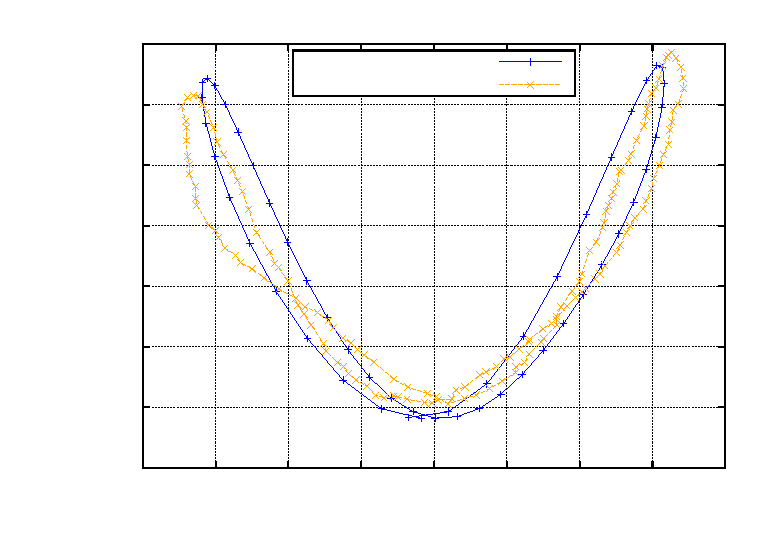
\includegraphics{CT1}}%
    \gplfronttext
  \end{picture}%
\endgroup
}
\end{minipage}
\caption{\label{fig1}Normal (left) and tangential (right) force coefficients during pitching motions of NACA0021 airfoil with a maximum amplitude of 17.4\degree\ (analog to $\lambda = 3.34$).}
\end{figure}


\begin{figure}[h]
\begin{minipage}{18pc}
%\includegraphics[width=18pc]{Fig3.png}
\resizebox{\columnwidth}{!}{% GNUPLOT: LaTeX picture with Postscript
\begingroup
  \makeatletter
  \providecommand\color[2][]{%
    \GenericError{(gnuplot) \space\space\space\@spaces}{%
      Package color not loaded in conjunction with
      terminal option `colourtext'%
    }{See the gnuplot documentation for explanation.%
    }{Either use 'blacktext' in gnuplot or load the package
      color.sty in LaTeX.}%
    \renewcommand\color[2][]{}%
  }%
  \providecommand\includegraphics[2][]{%
    \GenericError{(gnuplot) \space\space\space\@spaces}{%
      Package graphicx or graphics not loaded%
    }{See the gnuplot documentation for explanation.%
    }{The gnuplot epslatex terminal needs graphicx.sty or graphics.sty.}%
    \renewcommand\includegraphics[2][]{}%
  }%
  \providecommand\rotatebox[2]{#2}%
  \@ifundefined{ifGPcolor}{%
    \newif\ifGPcolor
    \GPcolorfalse
  }{}%
  \@ifundefined{ifGPblacktext}{%
    \newif\ifGPblacktext
    \GPblacktexttrue
  }{}%
  % define a \g@addto@macro without @ in the name:
  \let\gplgaddtomacro\g@addto@macro
  % define empty templates for all commands taking text:
  \gdef\gplbacktext{}%
  \gdef\gplfronttext{}%
  \makeatother
  \ifGPblacktext
    % no textcolor at all
    \def\colorrgb#1{}%
    \def\colorgray#1{}%
  \else
    % gray or color?
    \ifGPcolor
      \def\colorrgb#1{\color[rgb]{#1}}%
      \def\colorgray#1{\color[gray]{#1}}%
      \expandafter\def\csname LTw\endcsname{\color{white}}%
      \expandafter\def\csname LTb\endcsname{\color{black}}%
      \expandafter\def\csname LTa\endcsname{\color{black}}%
      \expandafter\def\csname LT0\endcsname{\color[rgb]{1,0,0}}%
      \expandafter\def\csname LT1\endcsname{\color[rgb]{0,1,0}}%
      \expandafter\def\csname LT2\endcsname{\color[rgb]{0,0,1}}%
      \expandafter\def\csname LT3\endcsname{\color[rgb]{1,0,1}}%
      \expandafter\def\csname LT4\endcsname{\color[rgb]{0,1,1}}%
      \expandafter\def\csname LT5\endcsname{\color[rgb]{1,1,0}}%
      \expandafter\def\csname LT6\endcsname{\color[rgb]{0,0,0}}%
      \expandafter\def\csname LT7\endcsname{\color[rgb]{1,0.3,0}}%
      \expandafter\def\csname LT8\endcsname{\color[rgb]{0.5,0.5,0.5}}%
    \else
      % gray
      \def\colorrgb#1{\color{black}}%
      \def\colorgray#1{\color[gray]{#1}}%
      \expandafter\def\csname LTw\endcsname{\color{white}}%
      \expandafter\def\csname LTb\endcsname{\color{black}}%
      \expandafter\def\csname LTa\endcsname{\color{black}}%
      \expandafter\def\csname LT0\endcsname{\color{black}}%
      \expandafter\def\csname LT1\endcsname{\color{black}}%
      \expandafter\def\csname LT2\endcsname{\color{black}}%
      \expandafter\def\csname LT3\endcsname{\color{black}}%
      \expandafter\def\csname LT4\endcsname{\color{black}}%
      \expandafter\def\csname LT5\endcsname{\color{black}}%
      \expandafter\def\csname LT6\endcsname{\color{black}}%
      \expandafter\def\csname LT7\endcsname{\color{black}}%
      \expandafter\def\csname LT8\endcsname{\color{black}}%
    \fi
  \fi
  \setlength{\unitlength}{0.0500bp}%
  \begin{picture}(7200.00,5040.00)%
    \gplgaddtomacro\gplbacktext{%
      \csname LTb\endcsname%
      \put(946,704){\makebox(0,0)[r]{\strut{}-2}}%
      \csname LTb\endcsname%
      \put(946,1213){\makebox(0,0)[r]{\strut{}-1.5}}%
      \csname LTb\endcsname%
      \put(946,1722){\makebox(0,0)[r]{\strut{}-1}}%
      \csname LTb\endcsname%
      \put(946,2231){\makebox(0,0)[r]{\strut{}-0.5}}%
      \csname LTb\endcsname%
      \put(946,2740){\makebox(0,0)[r]{\strut{} 0}}%
      \csname LTb\endcsname%
      \put(946,3248){\makebox(0,0)[r]{\strut{} 0.5}}%
      \csname LTb\endcsname%
      \put(946,3757){\makebox(0,0)[r]{\strut{} 1}}%
      \csname LTb\endcsname%
      \put(946,4266){\makebox(0,0)[r]{\strut{} 1.5}}%
      \csname LTb\endcsname%
      \put(946,4775){\makebox(0,0)[r]{\strut{} 2}}%
      \csname LTb\endcsname%
      \put(1078,484){\makebox(0,0){\strut{}-25}}%
      \csname LTb\endcsname%
      \put(1651,484){\makebox(0,0){\strut{}-20}}%
      \csname LTb\endcsname%
      \put(2223,484){\makebox(0,0){\strut{}-15}}%
      \csname LTb\endcsname%
      \put(2796,484){\makebox(0,0){\strut{}-10}}%
      \csname LTb\endcsname%
      \put(3368,484){\makebox(0,0){\strut{}-5}}%
      \csname LTb\endcsname%
      \put(3941,484){\makebox(0,0){\strut{} 0}}%
      \csname LTb\endcsname%
      \put(4513,484){\makebox(0,0){\strut{} 5}}%
      \csname LTb\endcsname%
      \put(5086,484){\makebox(0,0){\strut{} 10}}%
      \csname LTb\endcsname%
      \put(5658,484){\makebox(0,0){\strut{} 15}}%
      \csname LTb\endcsname%
      \put(6231,484){\makebox(0,0){\strut{} 20}}%
      \csname LTb\endcsname%
      \put(6803,484){\makebox(0,0){\strut{} 25}}%
      \put(176,2739){\rotatebox{-270}{\makebox(0,0){\strut{}$C_N$}}}%
      \put(3940,154){\makebox(0,0){\strut{}Angle of attack {$\alpha$} [$\degree$]}}%
    }%
    \gplgaddtomacro\gplfronttext{%
      \csname LTb\endcsname%
      \put(4437,4602){\makebox(0,0)[r]{\strut{}$C_N$ simulated}}%
      \csname LTb\endcsname%
      \put(4437,4382){\makebox(0,0)[r]{\strut{}$C_N$ experiments}}%
    }%
    \gplbacktext
    \put(0,0){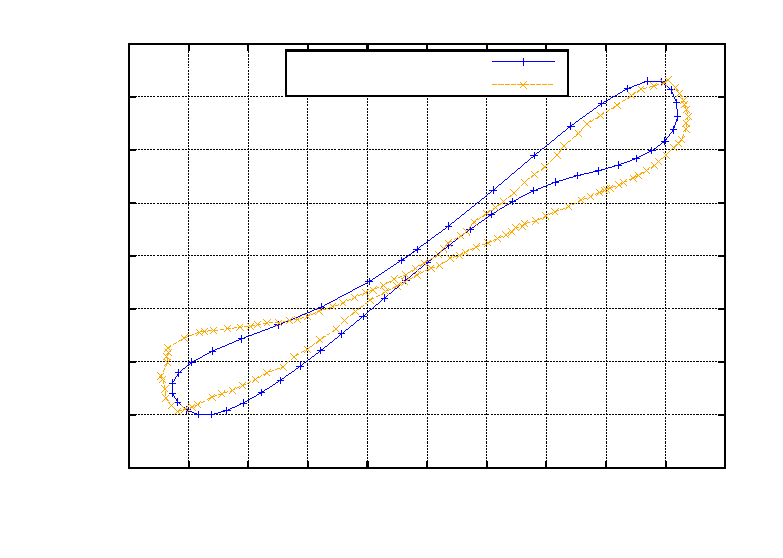
\includegraphics{CN2}}%
    \gplfronttext
  \end{picture}%
\endgroup
}
\end{minipage}\hspace{2pc}%
\begin{minipage}{18pc}
%\includegraphics[width=18pc]{Fig4.png}
\resizebox{\columnwidth}{!}{% GNUPLOT: LaTeX picture with Postscript
\begingroup
  \makeatletter
  \providecommand\color[2][]{%
    \GenericError{(gnuplot) \space\space\space\@spaces}{%
      Package color not loaded in conjunction with
      terminal option `colourtext'%
    }{See the gnuplot documentation for explanation.%
    }{Either use 'blacktext' in gnuplot or load the package
      color.sty in LaTeX.}%
    \renewcommand\color[2][]{}%
  }%
  \providecommand\includegraphics[2][]{%
    \GenericError{(gnuplot) \space\space\space\@spaces}{%
      Package graphicx or graphics not loaded%
    }{See the gnuplot documentation for explanation.%
    }{The gnuplot epslatex terminal needs graphicx.sty or graphics.sty.}%
    \renewcommand\includegraphics[2][]{}%
  }%
  \providecommand\rotatebox[2]{#2}%
  \@ifundefined{ifGPcolor}{%
    \newif\ifGPcolor
    \GPcolorfalse
  }{}%
  \@ifundefined{ifGPblacktext}{%
    \newif\ifGPblacktext
    \GPblacktexttrue
  }{}%
  % define a \g@addto@macro without @ in the name:
  \let\gplgaddtomacro\g@addto@macro
  % define empty templates for all commands taking text:
  \gdef\gplbacktext{}%
  \gdef\gplfronttext{}%
  \makeatother
  \ifGPblacktext
    % no textcolor at all
    \def\colorrgb#1{}%
    \def\colorgray#1{}%
  \else
    % gray or color?
    \ifGPcolor
      \def\colorrgb#1{\color[rgb]{#1}}%
      \def\colorgray#1{\color[gray]{#1}}%
      \expandafter\def\csname LTw\endcsname{\color{white}}%
      \expandafter\def\csname LTb\endcsname{\color{black}}%
      \expandafter\def\csname LTa\endcsname{\color{black}}%
      \expandafter\def\csname LT0\endcsname{\color[rgb]{1,0,0}}%
      \expandafter\def\csname LT1\endcsname{\color[rgb]{0,1,0}}%
      \expandafter\def\csname LT2\endcsname{\color[rgb]{0,0,1}}%
      \expandafter\def\csname LT3\endcsname{\color[rgb]{1,0,1}}%
      \expandafter\def\csname LT4\endcsname{\color[rgb]{0,1,1}}%
      \expandafter\def\csname LT5\endcsname{\color[rgb]{1,1,0}}%
      \expandafter\def\csname LT6\endcsname{\color[rgb]{0,0,0}}%
      \expandafter\def\csname LT7\endcsname{\color[rgb]{1,0.3,0}}%
      \expandafter\def\csname LT8\endcsname{\color[rgb]{0.5,0.5,0.5}}%
    \else
      % gray
      \def\colorrgb#1{\color{black}}%
      \def\colorgray#1{\color[gray]{#1}}%
      \expandafter\def\csname LTw\endcsname{\color{white}}%
      \expandafter\def\csname LTb\endcsname{\color{black}}%
      \expandafter\def\csname LTa\endcsname{\color{black}}%
      \expandafter\def\csname LT0\endcsname{\color{black}}%
      \expandafter\def\csname LT1\endcsname{\color{black}}%
      \expandafter\def\csname LT2\endcsname{\color{black}}%
      \expandafter\def\csname LT3\endcsname{\color{black}}%
      \expandafter\def\csname LT4\endcsname{\color{black}}%
      \expandafter\def\csname LT5\endcsname{\color{black}}%
      \expandafter\def\csname LT6\endcsname{\color{black}}%
      \expandafter\def\csname LT7\endcsname{\color{black}}%
      \expandafter\def\csname LT8\endcsname{\color{black}}%
    \fi
  \fi
  \setlength{\unitlength}{0.0500bp}%
  \begin{picture}(7200.00,5040.00)%
    \gplgaddtomacro\gplbacktext{%
      \csname LTb\endcsname%
      \put(946,1103){\makebox(0,0)[r]{\strut{} 0}}%
      \csname LTb\endcsname%
      \put(946,1901){\makebox(0,0)[r]{\strut{} 0.1}}%
      \csname LTb\endcsname%
      \put(946,2700){\makebox(0,0)[r]{\strut{} 0.2}}%
      \csname LTb\endcsname%
      \put(946,3498){\makebox(0,0)[r]{\strut{} 0.3}}%
      \csname LTb\endcsname%
      \put(946,4296){\makebox(0,0)[r]{\strut{} 0.4}}%
      \csname LTb\endcsname%
      \put(1078,484){\makebox(0,0){\strut{}-25}}%
      \csname LTb\endcsname%
      \put(1651,484){\makebox(0,0){\strut{}-20}}%
      \csname LTb\endcsname%
      \put(2223,484){\makebox(0,0){\strut{}-15}}%
      \csname LTb\endcsname%
      \put(2796,484){\makebox(0,0){\strut{}-10}}%
      \csname LTb\endcsname%
      \put(3368,484){\makebox(0,0){\strut{}-5}}%
      \csname LTb\endcsname%
      \put(3941,484){\makebox(0,0){\strut{} 0}}%
      \csname LTb\endcsname%
      \put(4513,484){\makebox(0,0){\strut{} 5}}%
      \csname LTb\endcsname%
      \put(5086,484){\makebox(0,0){\strut{} 10}}%
      \csname LTb\endcsname%
      \put(5658,484){\makebox(0,0){\strut{} 15}}%
      \csname LTb\endcsname%
      \put(6231,484){\makebox(0,0){\strut{} 20}}%
      \csname LTb\endcsname%
      \put(6803,484){\makebox(0,0){\strut{} 25}}%
      \put(176,2739){\rotatebox{-270}{\makebox(0,0){\strut{}$C_T$}}}%
      \put(3940,154){\makebox(0,0){\strut{}Angle of attack {$\alpha$} [$\degree$]}}%
    }%
    \gplgaddtomacro\gplfronttext{%
      \csname LTb\endcsname%
      \put(4437,4602){\makebox(0,0)[r]{\strut{}$C_T$ simulated}}%
      \csname LTb\endcsname%
      \put(4437,4382){\makebox(0,0)[r]{\strut{}$C_T$ experiments}}%
    }%
    \gplbacktext
    \put(0,0){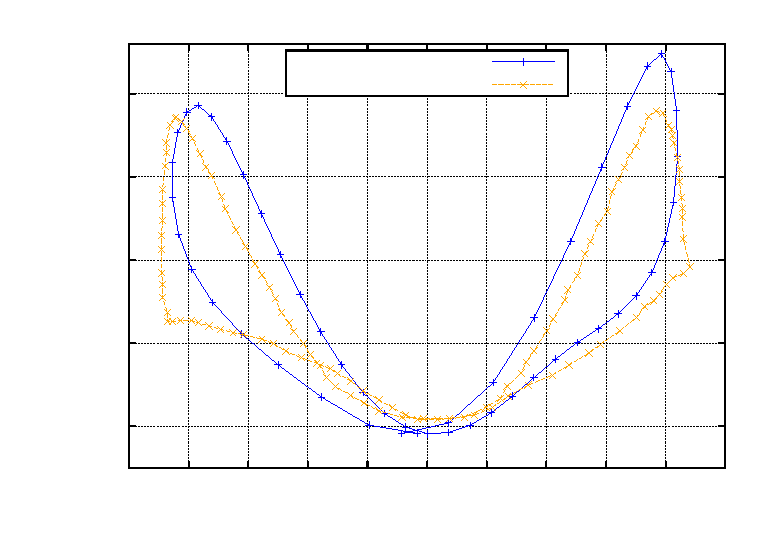
\includegraphics{CT2}}%
    \gplfronttext
  \end{picture}%
\endgroup
}
\end{minipage}
\caption{\label{fig2}Normal (left) and tangential (right) force coefficients during pitching motions of NACA0021 airfoil with a maximum amplitude of 22.6\degree\ (analog to $\lambda = 2.60$).}
\end{figure}

\newpage

\section{Results and discussion}

For a TSR of 3.34 (Figure \ref{fig1}), the maximum magnitude of the angle of attack is at
17.4\degree\ which is in the stall region. Both \textit{CN} and \textit{CT} curves show the delay
of the flow reattachment, which is characteristic of the dynamic stall
phenomenon. Peaks of simulated values have close agreement with the measured
data.

For a TSR of 2.60 (Figure \ref{fig2}), the maximum amplitude of the angle of attack is 22.6\degree, which
is related to a deeper stall region compared to a TSR of 3.34. This is shown
because the ``loop'' of the curve is wider for the lower TSR, and moreover, the
reattachment of the flow is further delayed.

In general, the model show good agreement with experimental data, considering the complexity
of the flows studied. This makes the model suitable for application in wind turbine
simulations.


\section*{References}
%\begin{thebibliography}{9}
%\bibitem{iopartnum} IOP Publishing is to grateful Mark A Caprio, Center for Theoretical Physics, Yale University, for permission to include the {\tt iopart-num} \BibTeX package (version 2.0, December 21, 2006) with  this documentation. Updates and new releases of {\tt iopart-num} can be found on \verb"www.ctan.org" (CTAN).
%\end{thebibliography}

\bibliography{mybib}{}
\bibliographystyle{unsrt}






\end{document}
